\chapter{模拟退火法}

之前我们的随机算法都有一个特性,即我们清楚随机变量的分布情况,能够用AR
法等手段进行服从指定分布的抽样,从而提高随机算法的效率和精度。同时,我
们的模拟目标往往是随机变量的某个数字特征,因此可以通过大数定律逼近。这
一章我们将随机算法扩展到优化领域。同时要面对上述前提失效的问题。本章的
内容基于参考书\cite{Kanglishan1994}。

\section{组合优化问题}
我们知道有很多离散优化问题,是
属于NP(Non-deterministic Polynomial )的,其中最著名的一个可能就是
TSP(Traveling Salesman Problem)问题,它的一种描述如下:给定$n$个城市
和每两个城市间的距离(无向完全图,有权边),选择一条线路,使得每个城市
只经过一次且仅有一次,并最终回到起点。求能完成这个遍历的总路径长度最短。
对于完全图,我们用邻接矩阵(adjacency matrix)$D = [d_{ij}]$来表示全部
城市,其中$d_{ij}$表示城市$i$和$j$之间的距离。显然,$d_{ij}$满足:
\begin{enumerate}
\item $d_{ij} \geq 0, 1 \leq i, j \leq n$;
\item $d_{ii} = 0, 1 \leq i \leq n$;
\item $d_{ij} = d_{ji}, 1 \leq i, j \leq n$;
\item $d_{ij} + d_{jk} \geq d_{ik}, 1 \leq i, j, k \leq n$.
\end{enumerate}
一个解可以表达为一个循环排列
$$
\pi = (\pi_1, \pi_2, \cdots, \pi_n),
$$
表示路径
$$
\pi_1 \to \pi_2 \to \cdots \to \pi_n,
$$
其中$\pi_i \in \{1, 2, \cdots, n\}, i = 1, 2, \cdots, n$表示各个城市
的编号,显然对可行解,有$i \neq j$,有$\pi_i \neq \pi_j$。若记$S$为全体
可行解,则易知
\begin{equation}
  |S| = \frac{(n - 1)!}{2},
\end{equation}
这是一个随$n$增加指数增长的数值,因此对于较大的$n$不太可能用遍历穷举的
方式来寻找最优解。这里目标函数可以表示为
\begin{equation}
  f(\pi) = \sum_{i = 1}^n d_{\pi_i, \pi_{i + 1}},
\end{equation}
这里约定$\pi_{n + 1} = \pi_1$。整个优化问题按组合优化的约定,可以表达为
\begin{equation}
  \min f(\pi_i), \pi_i \in S.
\label{eq::TSP_opt}
\end{equation}
而优化问题(\ref{eq::TSP_opt})的解则定义为:

\begin{definition}{\hei 全局最优解} 称$\pi^* \in S$为问题(\ref{eq::TSP_opt})
  的全局最优解,或简称最优解,若$\forall \pi_i \in S$,有
  $$
   f(\pi^*) \leq f(\pi_i).
  $$
\end{definition}

作为一个典型的NP问题,对每一个可行解(存在的路径),我们都可以迅速得到
总路径长度(多项式时间)。然而,求最短路径本身却至今没有什么太好的确定
性算法。在这种情况下,随机搜索算法又一次被提到桌面上讨论。然而现在出现
新的困难,和积分问题不同,最优解是一个非常孤立的偶然事件,同时分布上也
没有明显的规律(或者我们无法先验地获知它的分布情况),如果完全在$S$全
空间随机投点,去碰一个偶然事件,那么收敛速度甚至收敛性本身都很有问题。
针对这种未知分布的情况,我们得改变我们的抽样技巧。但首先,我们先观察一
下$S$的结构(总是要尽可能获取背景信息)。

\begin{definition}{\hei $2$-变换邻域}
对于$S$中的一个解
$$
\pi = \{\pi_1, \pi_2, \cdots, \pi_{p - 1}, \pi_p, \pi_{p + 1},
\cdots, \pi_{q - 1}, \pi_q, \pi_{q + 1}, \cdots, \pi_n\},
$$
称
$$
N_2(p, q): \pi \to \pi', p < q
$$
为$2$-变换,如果
$$
\pi'= \{\pi_1, \pi_2, \cdots, \pi_{p - 1}, \pi_q, \pi_{q - 1},
\cdots, \pi_{p + 1}, \pi_p, \pi_{q + 1}, \cdots, \pi_n\}.
$$
$\forall \pi_i \in S$,称$S_i$为$\pi_i$的$2$-变换邻域,若$S_i \subseteq S$,
且$\forall \pi_j \in S_i$,$\pi_j$可由$\pi_i$经一次$2$-变换得到。
\end{definition}

类似的,我们还可以定义$k$-变换,以及$k$-变换邻域。但注意到$\forall i,
j \in S$,我们都可以用至多$n - 2$次$2$-变换将二者互换。所以从考虑可行
解之间关系角度,$2$-变换在很多场合也够用了。有了邻域,我们可以进一步提出:

\begin{definition}{\hei 局部最优解}
  记$\pi^* \in S$的邻域为$S^*$,若$\forall \pi_i \in S^*$,有
  $$
  f(\pi_i) \geq f(\pi^*), 
  $$
  则称$\pi^*$为优化问题(\ref{eq::TSP_opt})的局部最优解。
\end{definition}

现在我们给出一个用于求解一般组合优化问题的伪代码:

\begin{minipage}[!ht]{0.8\textwidth}
\vspace{3ex}
\refstepcounter{alg}
\label{alg::LSA}
\begin{center}
 算法 \arabic{chapter}.\arabic{alg} {\hei 组合优化问题的局部搜索算法} 
\end{center}
\small
\begin{tabular}{lll}
  \hei 输入&i0&初值\\
  \hei 输出&&局部最优解
\end{tabular}
\begin{lstlisting}[style = python]
def local_search(i0):
    i = i0
    while (i不是局部最优解):
        从i的邻域Si中选取一个可行解j
        if f(j) < f(i):
            i = j
    return i
\end{lstlisting}
\end{minipage}

这个算法很通用,但也很没用。它只能提供局部最优解,对于TSP这样显然要求
全局最优的问题,它显得很无力。(TSP算法有实用的离散算法,详见谈之奕主
  讲课程《组合优化》。)我们这里考虑能否使用随机搜索的手段,使这个算法
摆脱局部最优解的困扰,但同时我们又要利用局部最优性。因为在没有其他任何
信息的时候,局部最优性显然提供了一个邻域内的有效索方向。这里可以考虑的
几个关键点是:
\begin{enumerate}
  \item 我们在邻域内每次都做一个随机选取,即总是从$S_i$中随机抽取一个
    $j$,作为下一步尝试的可行解。比如具体在TSP问题中,可以通过随机抽取
    $p$和$q$来进行$2-$变换邻域内的随机抽取;
  \item 当存在邻域内的可行解$j$满足$f(j) > f(i)$时,也应该有一定概率用
    $j$去代替$i$,也就是说应该保留一定概率让解往非局部最优的方向行走,
    这样才能留下脱离局部最优解的可能性。具体这个概率应该服从什么分布?
    这个是我们接下去要讨论的问题;
  \item 在引入了上述随机搜索之后,算法\ref{alg::LSA}的终止判定不再适用,
    应该相应修改为若当前解$i$在一个指定的步数$N$($N >> 1$)都不再变化
    时,算法终止。
\end{enumerate}

由于缺乏关键过程2,我们现在还无法写出这个算法,但大致思想框架已经形成。

\section{Metropolis准则}

Metropolis是一个人名,他是一个物理学家。由于工作的缘故,他是首批接触到
计算机的人之一,因此也为计算机模拟计算的早期研究作出了杰出贡献。当时的
计算机还非常低效,不太可能进行高维大范围的随机抽样。而Metropolis在求解
一组原子结构的最低能量状态时,提出了后来被称为Metropolis准则的模拟方法。

\begin{figure}[!ht]
\centering
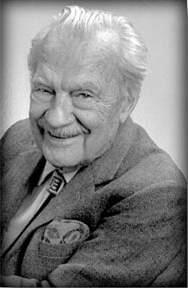
\includegraphics[width=0.3\textwidth]{images/Nicholas.PNG}
\caption{Nicholas Metropolis,1915 - 1999,希腊裔美国物理学家,曼哈顿
  计划的参与者}
\label{fig::game}
\end{figure}

物质在从液态变成固态时,系统的能量是整体降低的。粒子(我们这里不区分原
  子、分子)从能流动到被固定在一个有限范围振动,物质的结构性加强,
能量降低,熵减少。这里温度是刻画粒子状态的一个统计量。在宏观意义上,它
和粒子系统的能量是正相关的。同时在宏观上,我们可以通过控制外界温度,来
影响系统的温度,进而影响系统状态。比如对于液体,我们降低温度,它会凝固
成固体。这一过程称为退火。实践和理论研究都指出,温度降低的过程对最终形
成的固体的性态是有影响的。如果温度急剧下降,那么粒子系统来不及和周围环
境进行充分的能量交换,从而导致粒子尚未进入到能量最低态就进入固体状态,
因此形成的固体物质结构较为脆弱。而如果能控制温度缓慢下降,使粒子系统整
体能量和外界交换均匀充分,那么粒子系统能量降低到一个最低值时,趋于稳定,
此时形成的固体,结构更加坚固。物理学家通过理论分析和实验,得到一系列关
于物质能量和熵条件的结果,我们这里不再详述,有兴趣同学自行阅读参考书。
而1953年Metropolis在前人工作的基础上,提出了一种用于模拟系统能量最低态的
随机采样准则:若系统在状态$i$时的能量为$E_i$,在$i$的邻域内随机选取
$j\neq i$,且状态$j$的能量为$E_j$。若$E_j < E_i$,则称状态$j$为“重要
状态”,否则,若$E_j > E_i$,则以
\begin{equation}
  r = e^{\frac{E_i - E_j}{kT}}
  \label{eq::Metropolis}
\end{equation}
的概率决定$j$是否为重要状态。也就是说,产生一个服从$U(0, 1)$的随机数
$\xi$,若$\xi < r$,则接受$j$为重要状态,否则舍弃。在一次随机尝试中,
如果$j$是重要状态,则用$j$代替$i$成为当前状态。公式
(\ref{eq::Metropolis})来源于统计物理学中的Gibbs分布,而$k$是
Boltzmann常数,而$T$是温度。受到启发,Kirkpatrick在1983年
\cite{KirkpatrickGelattVecchi83}将这种基于物质退火过程模拟的思
想引入了组合优化领域,提出了模拟退火算法(Simulated Annealing Algorithm)。回顾我们之前考虑局部随机搜索算法时尚未解决的
第2步,即解$i$应该以怎样的概率转移到解$j$?根据模拟退火法,这个转移概
率可以写作:
\begin{equation}
  P_t\{i \to j\} = \left\{
  \begin{array}{ll}
    1, & f(j) \leq f(i)\\
    e^{\frac{f(i) - f(j)}{t}}, &\mbox{其它}.
  \end{array}
  \right.
  \label{eq::SAA_metro}
\end{equation}
这里将所有参数吸收为一个$t > 0$,显然$t$越大,则转移概率越高;而$t$越
小,转移概率越低。这与物质退火的直观一致。我们在执行算法时,可以在初期
将$t$设的较大,然后慢慢降低$t$,最终使状态最终在一个能量低点稳定。

现在我们可以给出基于Metropolis准则的随机局部搜索算法,也即模拟退火算法
的伪代码。

\begin{minipage}[!ht]{0.8\textwidth}
\vspace{3ex}
\refstepcounter{alg}
\label{alg::SA}
\begin{center}
 算法 \arabic{chapter}.\arabic{alg} {\hei 模拟退火算法} 
\end{center}
\small
\begin{tabular}{lll}
  \hei 输入&i0&初值\\
  &t0&初始温度\\
  &L0&初始随机搜索步长,即在初始温度下的随机搜索次数。\\
  \hei 输出&&数值最优解
\end{tabular}
\begin{lstlisting}[style = python]
def simulated_annealing(i0, t0, L0):
    k = 0
    i = i0
    while (1):
        for l = 1 to Lk:
            从i的邻域Si中选取一个可行解j
            if f(j) < f(i):
                i = j
            else:
                xi = random(0, 1)
                if xi < exp((f(i) - f(j))/tk):
                    i = j
        k = k + 1
        调整Lk
        调整tk
        若满足终止条件,跳出循环
    return i
\end{lstlisting}
\end{minipage}

这仍然只是一个框架式算法思路。如何调整Lk,tk,以及如何制定终止条件,既
有理论上的讨论,也要根据实际问题具体分析。但我们这里先给出一个关于模拟
退火法的收敛性的统计学特性。

\begin{definition}{\hei 平稳分布}
  给定组合优化问题$(S, f)$,和一个相关的邻域结构。对固定的$t$值做足够
  多的基于Metropolis准则(\ref{eq::SAA_metro})变换之后,全体可行解的
  分布服从
  \begin{equation}
    P\{X = i\} := q_i(t) = \frac{e^{-\frac{f(i)}{t}}}{N_0}
    \label{eq::Metro_Gibbs_dis}
  \end{equation}
  其中$X$是表示当前解的随机变量,而
  \begin{equation}
    N_0(t) = \sum_{i \in S} e^{-\frac{f(j)}{t}}
    \label{eq::Metro_Gibbs_dis_regular}
  \end{equation}
  是归一化因子。式(\ref{eq::Metro_Gibbs_dis})称为平稳分布。
\end{definition}
模拟退火法的当前解服从平稳分布是一个假设。在这个假设下,我们有

\begin{theorem}{}
  若组合优化问题$(S, f)$的当前解服从平稳分布,则
  \begin{equation}
    \lim_{t \to 0}q_i(t) := q_i^* = \frac{1}{|S_{\mathrm{opt}}|}\chi_{\mathrm{opt}}.
  \end{equation}
  其中$S_{\mathrm{opt}}$表示最优解集合(不唯一),而$\chi_{\mathrm{opt}}$
  则表示可行解$i$是最优解的特征函数:
  \begin{equation}
    S \to \{0, 1\}, \chi_{\mathrm{opt}}(i) = \left\{\begin{array}{ll}
    1, & i \in S_{\mathrm{opt}},\\
    0, &\mbox{其它}.
    \end{array}\right.
  \end{equation}
\end{theorem}

这个定理表明,如果每个$t$至都能达到平稳分布,那么算法能收敛到全局最优解。先看证明。

\begin{proof}
  对$\forall a \geq 0$,有
  \begin{equation}
    \lim_{x \to 0} e^{\frac{a}{x}} = \left\{
    \begin{array}{ll}
      1, & a = 0,\\
      0, & a < 0.
    \end{array}
    \right.
  \end{equation}
  所以
  \begin{eqnarray*}
    \lim_{t \to 0}q_i(t) & = & \lim_{t \to 0}  \frac{e^{-\frac{f(i)}{t}}}
        {\sum_{j \in S} e^{-\frac{f(j)}{t}}} \\
        & = & \lim_{t \to 0} \frac{\frac{e^{f_{\mathrm{opt}} - f(i)}}{t}}
        {\sum_{j \in S} e^{\frac{f_{\mathrm{opt}} - f(j)}{t}}} \\
        & = & \lim_{t \to 0}\frac{1}{\sum_{j \in S} e^{\frac{f_{\mathrm{opt}} - f(j)}{t}}}
        \chi_{\mathrm{opt}}(i)
        + \lim_{t \to 0} \frac{e^{\frac{f_{\mathrm{opt}} - f(i)}{t}}}
        {\sum_{j \in S}e^{\frac{f_{\mathrm{opt}} - f(j)}{t}}}\chi_{\mathrm{opt}}(i)\\
        & = & \frac{1}{|S_{\mathrm{opt}}|} \chi_{\mathrm{opt}}(i) + 0. 
  \end{eqnarray*}
\end{proof}

下面列出一些关于模拟退火法的重要统计学特征,具体的证明参见文献\cite{Aarts1989Simulated}。

\begin{definition}{\hei 平衡时的期望目标函数}
  \begin{equation}
    E_t(f) := \langle f \rangle_t = \sum_{i \in S}f(i)q_i(t).
    \label{eq::Metro_esp_t_f}
  \end{equation}
\end{definition}

\begin{definition}{\hei 平衡时的期望平方目标函数}
  \begin{equation}
    E_t(f^2) := \langle f^2\rangle_t = \sum_{i \in S}f^2(i)q_i(t).
    \label{eq::Metro_esp_t_f2}
  \end{equation}
\end{definition}

\begin{definition}{\hei 平衡时的目标函数方差}
  \begin{equation}
    Var_t(f) := \sigma_t^2 = \sum_{i \in S}(f(i) - \langle f\rangle_t)^2q_i(t)
    = \langle f^2\rangle_t - \langle f\rangle_t^2.
    \label{eq::Metro_t_variation}
  \end{equation}
\end{definition}

\begin{definition}{\hei 平衡时的熵}
  \begin{equation}
    S_t(f) := \sum_{i \in S} q_i(t) \log q_i(t).
    \label{eq::Metro_t_entropy}
  \end{equation}
\end{definition}

\begin{theorem}{}
  \begin{equation}
    \frac{\partial}{\partial t}\langle f\rangle_t = \frac{\sigma_t^2}{t^2},
  \end{equation}
  \begin{equation}
    \frac{\partial}{\partial t}S_t = \frac{\sigma_t^2}{t^3},
  \end{equation}
\end{theorem}

\begin{theorem}{}
  \begin{equation}
    \lim_{t \to \infty} \langle f\rangle_t := \langle f\rangle_\infty
    = \frac{1}{|S|}\sum_{i \in S} f(i).
  \end{equation}
  \begin{equation}
    \lim_{t \to 0} \langle f\rangle_t := f_{\mathrm{opt}}.
  \end{equation}
  \begin{equation}
    \lim_{t \to \infty} \sigma_t^2 := \sigma_\infty^2 = \frac{1}{|S|}
    \sum_{i \in S}(f(i) - \langle f\rangle_\infty)^2.
  \end{equation}
  \begin{equation}
    \lim_{t \to 0} \sigma_t^2 = 0.
  \end{equation}
  \begin{equation}
    \lim_{t \to \infty} S_t := S_\infty = \log |S|.
  \end{equation}
  \begin{equation}
    \lim_{t \to 0} S_t := S_0 = \log |S_{\mathrm{opt}}|.
  \end{equation}
\end{theorem}

有上述定理可知,若在每个$t$时刻都能满足平稳分布,则模拟退火法的期望目
标函数和熵分别单调减少至$f_{\mathrm{opt}}$和$\log |S_{\mathrm{opt}}|$.

\begin{theorem}{} 设$(S, f)$表示某个组合优化问题,
  且$S_{\mathrm{opt}} \neq S$(非平凡). 并设$q_i(t)$为相关$t$时刻平稳分布,则
  \begin{enumerate}
  \item $\forall i \in S_{\mathrm{opt}}$,有
    \begin{equation}
      \frac{\partial}{\partial t}q_i(t) < 0;
    \end{equation}
  \item $\forall i \notin S_{\mathrm{opt}}$, $f(i) \geq \langle f\rangle_\infty$,有
    \begin{equation}
      \frac{\partial}{\partial t} q_t(i) > 0;
    \end{equation}
  \item $\forall i \notin S_{\mathrm{opt}}$, $f(i) < \langle f\rangle_\infty$,则
    $\exists \tilde{t}_t > 0$, 使
    \begin{equation}
      \frac{\partial}{\partial t} q_i(t) \left\{
      \begin{array}{ll}
        > 0, & t < \tilde{t}_i, \\
        = 0, & t = \tilde{t}_i, \\
        < 0, & t > \tilde{t}_i.
      \end{array}
      \right.
    \end{equation}
  \end{enumerate}
  \label{thm::Metro_q_t}
\end{theorem}

由定理\ref{thm::Metro_q_t}知,模拟退火法找到一个整体最优解的概率随$t$
的减少而单调增大;且对每个非整体最优解,都存在$\tilde{t}_i$,使得当$t
< \tilde{t}_i$时,当前解为该解的概率随$t$的减少而单调减少。

\section{Markov链理论}

Markov是俄国数学家,他以提出Markov链理论而闻名。

\begin{definition}{\hei \bf Markov链} 如果一个尝试序列(随机变量序列)的
  第$k$次结果仅受第$k - 1$次结果的影响,我们称这个尝试序列为Markov链。设
  $X(k)$为该序列的第$k$次结果的随机变量,则对于每对结果$i$和$j$,第$k$次
  尝试时的转移概率(也即在第$k$次尝试时恰好发生从结果$i$转移到结果$j$的
    概率)定义为
  \begin{equation}
    P_{ij}(k) = P\{(X(k) = j) | X(k - 1) = i\}.
  \end{equation}
  称矩阵$P(k) = [P_{ij}(k)]$为转移矩阵。
\end{definition}
若用$a_i(k)$表示第$k$次尝试结果为$i$的概率,即
\begin{equation}
  a_i(k) = P\{X(k) = i\},
\end{equation}
则显然
\begin{equation}
  a_i(k) = \sum_{l} a_l(k - 1)P_{li}(k).
\end{equation}

\begin{definition}{\hei \bf 有限Markov链} 如果
  一个Markov链的全部可能结果是一个有限集,则称为有限(finite)Markov链。
\end{definition}

\begin{definition}{\hei \bf 齐次Markov链} 如果转移概率$P_{ij}(k)$
  与$k$无关(关于尝试次数$k$是个常数),那么称为齐次(homogeneous)Markov链;
  反之,称为非齐次的(inhomogenous)。
\end{definition}

下面约定对于随机向量$\vec{a}$,总满足
\begin{equation}
  \sum_i a_i = 1, \mbox{且全部分量}~a_i \geq 0.
\end{equation}
对随机矩阵$P$亦有
\begin{equation}
  \sum_{i, j}P_{ij} = 1, \mbox{且全部元素}~P_{ij} \geq 0.
\end{equation}

对于模拟退火算法,显然,一次尝试对应于一次变换,且全部可能的结果是一个
有限集。并且每一次变换的结果仅受前一次尝试的结果的影响。因此我们面对的
实际是一个有限Markov链问题。具体来看,对一个组合优化问题$(S, f)$,定义
转移概率为:

\begin{equation}
  P_{ij}(k) = P_{ij}(t_k) = \left\{
  \begin{array}{ll}
    \displaystyle G_{ij}(t_k)A_{ij}(t_k), &i \neq j,\\\\
    \displaystyle 1 - \sum_{l \in S, l \neq i} P_{il}(t_k), &i = j,
  \end{array}  
  \right. \forall i, j \in S.
\end{equation}
其中,$G_{ij}(t_k)$表示产生概率,即从结果$i$产生结果$j$的概率,定义为:
\begin{equation}
  G_{ij}(t_k) = G_{ij} = \frac{1}{|S_i|}\chi_{S_i}(j), \forall i, j \in S.
\end{equation}
特别地,若对$\forall i \in S$,有$|S_i| = \Theta$, 则
\begin{equation}
  G_{ij} = \frac{1}{\Theta} \chi_{S_i}(j).
\end{equation}
而$A_{ij}(t_k)$成为接受概率,即一旦从$j$产生了结果$i$,被接受为下一步
结果的概率,定义为:
\begin{equation}
  A_{ij}(t_k) = e^{-\frac{(f(j) - f(i))^+}{t_k}}, \forall i, j \in S.
\end{equation}
这里,
\begin{equation}
  a^+ = \left\{
  \begin{array}{ll}
    a, & a > 0,\\
    0, & a \leq 0.
  \end{array}
  \right.
\end{equation}

注意接受矩阵不满足归一性。上述的定义主要考虑了模拟退火算法在物理中的背
景。接下去我们分别在齐次和非齐次的情形下讨论模拟退火法的收敛性。

首先是齐次情形,为此,可令$t_k = t$,转移矩阵$P(k) = P$。那么以$P$为转
移矩阵的平稳分布(稳定分布,分布不再变化)定义为向量$\vec{q}$,其中第
$i$个分量$q_i$为
\begin{equation}
  q_i = \lim_{k \to \infty}P\{X(k) = i | X(0) = j\}.
  \label{eq::station_vec}
\end{equation}
若这样的分布$\vec{q}$存在,则
\begin{eqnarray*}
  \lim_{k \to \infty} a_i(k) & = & \lim_{k \to \infty} P\{X(k) = i\} \\
  & = & \lim_{k \to \infty} \sum_j P\{X(k) = i | X(0) = j\}P\{X(0) = j\} \\
  & = & q_i \sum_{j} P\{X(0) = j\} = q_i.
\end{eqnarray*}
即这样定义的确实是$k \to \infty$的稳态分布。

再令
\begin{equation}
  a_i(0) = P\{X(0) = i\},
\end{equation}
则
\begin{eqnarray*}
  \vec{q}^T & = & \lim_{k \to \infty} \vec{a}^T(0) \prod_{l = 1}^k P(l)
  = \lim_{k \to \infty} \vec{a}^T(0) P^k \\
  & = & \lim_{k \to \infty} \vec{a}^T(0)P^{k - 1}P
  = \lim_{l \to \infty}\vec{a}^T(0)P^lP \\
  & = & \vec{q}^TP.
\end{eqnarray*}
因此,事实上,$\vec{q}$就是转移矩阵$P$特征值为$1$的特征向量。因此我们
只要对$P$提出足够的条件,就能确保$\vec{q}$的存在性。

\begin{definition}{\hei \bf 不可约Markov链} 如果转移矩阵为$P$的Markov链满足:
  \begin{equation}
    \forall i, j \in S, \exists n \geq 1 : (P^n)_{ij} > 0.
  \end{equation}
  则称该Markov链为不可约的(irreducible)。
\end{definition}
也即在充分多次尝试后,不可约Markov链的任何解对$i$和$j$都有机会互相转换。

\begin{definition}{\hei \bf 非周期Markov链} 如果转移矩阵为$P$的Markov链满足:
  $\forall i \in S$,由正整数组成的集合$D_i$的最大公约数为:
  \begin{equation}
    \gcd(D_i) = 1
  \end{equation}
  其中$D_i$为所有满足
  \begin{equation}
    (P)^n_{ii} > 0.
  \end{equation}
  的正整数$n$构成。则称该Markov链是非周期的(aperiodic)。称$\gcd(D_i)$为解$i$的周期。
\end{definition}
有周期性的Markov链本质上是不对称的,我们希望的Markov链是彻底的随机游走,
不带任何历史记忆。

这两个定义之间的联系可以参考以下这个引理:

\begin{lemma}{}
  转移矩阵为$P$的不可约Markov链是非周期的,若$\exists j \in S$满足$P_{jj} > 0$。
  \label{lemma::aperiodic_de}
\end{lemma}
也即只要转移矩阵中有一个状态能在一步回返。

\begin{proof}
  由不可约性知,对满足$P_{jj} > 0$的$j$和$\forall i \in S$,$\exists k, l \geq 1$,
  使得$(P^k)_{ij} > 0$和$(P^l)_{ji} > 0$。故对$n = k + l$,有
  $$
  (P^n)_{ii} \geq (P^k)_{ij}(P^l)_{ji} > 0.
  $$
  而对于$n + 1$,亦有
  $$
  (P^{n + 1})_{ii} \geq (P^k)_{ij}P_{jj}(P^l)_{ji} > 0,
  $$
  因此$n ,n + 1 \in D_i$,即
  $$
  \gcd(D_i) \leq gcd(n, n + 1) = 1.
  $$
  而$\gcd(D_i) \geq 1$,故$\gcd(D_i) = 1$。
\end{proof}

\begin{theorem}{\bf Feller, 1950 \cite{Feller1950An}} 令$P$为有限齐次Markov链的转移矩阵,
  且该Markov链是不可约和非周期的,则存在满足(\ref{eq::station_vec})的向量$\vec{q}$,且
  $\forall i, q_i$由方程
  \begin{equation}
    \sum_jq_jP_{ji} = q_i.
  \end{equation}
  唯一确定。这里$q_i > 0$且$\sum_i q_i = 1$。
\end{theorem}


联系到具体的模拟退火算法,则有:

\begin{lemma}{} 与模拟退火法相伴的Markov链是不可约的,若$\forall i, j \in S$,
  $\exists P \geq 1$以及$l_0 = i, l_1, \cdots, l_p = j \in S$,使得
  \begin{equation}
    G_{l_kl_{k + 1}} > 0, k = 0, 1, \cdots, P - 1.
  \end{equation}
\end{lemma}
也即任何两个解之间经过充分多次变换可以转变。这个只是将两个定义对接一下。证明略。进而有:

\begin{lemma}{} 若与模拟退火法相伴的Markov链是不可约的,且
  $\forall t > 0$,$\exists i_t, j_t \in S$满足$A_{i_tj_t}(t) < 1$,
  则该Markov链是非周期的。
\end{lemma}
这个引理表明只要在任何时刻,都至少还有一对解$i_t$和$j_t$之间的状态转换不是必然的,
这个隐含的意义是解空间$S$不是平凡的。

\begin{proof}
  注意到$\forall i, j \in S$,有$A_{ij} \leq 1$,由$A_{i_tj_t}(t) < 1$,得:
  \begin{eqnarray*}
    P_{i_ti_t}(t) & = & 1 - \sum_{l \in S, l \neq i_t} G_{i_tl}A_{i_tl}(t) \\
    & = & 1 - G_{i_tj_t}A_{i_tj_t}(t) - \sum_{l \in S, l \neq i_t, j_t} G_{i_tl}A_{i_tl}(t) \\
    & > & 1 - G_{i_tj_t} - \sum_{l \in S, l \neq i_t, j_t}G_{i_tl} \\
    & = & 1 - \sum_{l \in S, l \neq i_t} G_{i_tl} \geq 0.
  \end{eqnarray*}
  再由引理\ref{lemma::aperiodic_de}得证。
\end{proof}

\begin{corollary}{} 设$P$为有限齐次不可约非周期Markov链的转移矩阵,则该Markov链的平稳分布
  向量$\vec{q}$的分量满足$\forall i, j \in S$,
  \begin{equation}
    q_i P_{ij} = q_j P_{ji}.
  \end{equation}
\end{corollary}
该推论事实上提供了一种利用局部行为判断当前是否已经达到平稳分布的可能。

由此,我们已经可以判定,对于齐次Markov链,在不可约和非周期的前提下,对
充分大的$k$,能确保达到平稳分布。结合前一节分析,相应的组合优化问题能
达到全局最优解。对于非齐次Markov链,也有类似结论,有兴趣同学自行参考
\cite{Aarts1989Simulated}中相关内容。然而,这个结论并不是特别正面,因
为充分大基本意味我们的计算时间要趋于无穷。这对实际问题是没有意义的。因
此在实际应用中,我们会从实际情况出发,去寻求最优解的一个逼近,同时对计
算代价也给出一个具体的上界限制。

\section{冷却进度表}
在实际计算中,模拟退火法有几个重要参数需要决定:初始温度$t_0$,终止温
度$t_f$,温度衰减函数$t_k$,以及在每个温度的变换次数或Markov链长度
$L_k$。上一节的分析给我们提供了一些理论上的依据和直观,这一节我们面向
具体问题来讨论如何确定这些参数。

\subsection{初始温度$t_0$}
确定$t_0$的基本出发点,从Markov链出发,我们希望$t_0$基本上是一个无
条件准平衡状态。也希望即初始接受率
\begin{equation}
  \chi_0 = \frac{\mbox{接受变换数}}{\mbox{提出变换数}} \approx 1.
\end{equation}
只有这样,我们才能在算法运行初期充分遍历整个可行解空间,发掘潜在的最优解。
在这个前提下,根据Metropolis准则
$$
e^{-\frac{\Delta f}{t_0}} \approx 1,
$$
知,$t_0$应取得较大。或者可以根据需要的$\chi_0$反向推导$t_0$。比如如
果知道$\Delta f$的上界为$100$,且要求$\chi_0 = 0.9$,则可取$t_0 > 949$。
但如果缺乏对$\Delta f$的必要估计,那么也可以用具体的算法过程来控制,比
如,Kirkpatrick 1982(83?)提出,可以先确定一个初始$t_0$,然后做几次尝
试变换,若接受率不足,则将$t_0$翻倍,如此循环直到$t_0$满足要求。除此以
外还有大量文献讨论这个问题。

\subsection{终止温度$t_f$}
一种暴力的做法是限制$k$的次数,比如$k$至多$50$次。这种限制主要来自硬件。
而从理想角度出发,终止温度恰好和初始温度相反,我们希望它充分小。或者,
接受率$\chi_f$充分小。为此可以分别设置阈值,当$t_k$或$\chi_k$达到时,
就终止算法。而一种更硬核的思路是在连续一个或若干个Markov链中,最优解都
没有任何变化。Kirkpatrick本人就持这种观点。

\subsection{Markov链长度$L_k$}
也即在一个$t_k$温度下我们应该迭代多少次。理想的做法当然是迭代到平稳分
布,或者至少利用局部信息监测到平稳分布的发生。但这样的算法往往是指数时
间的。于是更常用的做法是设置一个多项式的上界$\bar{L}$,一旦达到,就不
再在此温度继续尝试。比如对TSP问题,一个常用的上界是$\bar{L} = n^2$,这
里$n$指解空间规模$|S|$。

\subsection{温度衰减函数$t_k$}
一个最常用的衰减函数是
\begin{equation}
  t_{k + 1} = \alpha \cdot t_k, k = 0, 1, \cdots
\end{equation}
其中$\alpha$接近$1$,比如$\alpha = 0.95$。(别问为什么!)
而稍微有节操一点的做法,比如
\begin{equation}
  t_k = \frac{K - k}{K} \cdot t_0, k = 1, 2, \cdots, K.
\end{equation}
这个策略事实上和前面的有限步终止温度是配套的。

以上种种,都是开放问题,在每一个具体问题中,都需要基于上述思路去进行调
整。目前在整个领域中,都没有明显的理论最优值可以提供。因此每年还在源源
不断地产生大量的论文。大家如果在SRTP或者毕业设计中有需要,不妨也考虑一
下,不过指导教师建议大家去找更专业的老师。